Laut \S 2 Nr. 8 SigG können Zertifizierungsstellen von natürlichen und juristischen Personen betrieben werden. Der Betrieb einer Zertifizierungsstelle ist grundsätzlich genehmigungsfrei, obliegt dennoch folgenden Bestimmungen nach \S 4 SigG. Der Betrieb einer Zertifizierungsstelle setzt Fachkunde, Zuverlässigkeit, Deckungsvorsorge gemäß \S 12 SigG gegen Schadenersatzansprüche voraus. Des Weiteren ist die Erfüllung der Sicherheitsansprüche anhand eines von der Prüfstelle abgenommenen Sicherheitskonzepts notwendig. "'Die erforderliche Fachkunde liegt vor, wenn die im Betrieb eines Zertifizierungsdienstes tätigen Personen über die für diese Tätigkeit notwendigen Kenntnisse, Erfahrungen und Fertigkeiten verfügen"' \footnote{\S 4 Abs. 2 Satz 3 Signaturgesetz \cite{grundlagenFN2}}. "'Die erforderliche Zuverlässigkeit besitzt, wer die Gewähr dafür bietet, als Zertifizierungsdiensteanbieter die für den Betrieb maßgeblichen Rechtsvorschriften einzuhalten"' \footnote{\S 4 Abs. 2 Satz 2 Signaturgesetz \cite{grundlagenFN2}}. Als Trust Center bezeichnet man die Einrichtungen, die die Verschlüssung von Daten anbieten und das Hochsicherheitsrechenzentrum betreiben. Zertifizierungsstellen und Trust Center werden benötigt, wenn eine große Anzahl von Benutzern am digitalen Signaturverfahren teilnehmen. Die Hauptaufgabe der Zertifizierungsstelle ist die Identifizierung der Antragssteller für einen Signaturschlüssel mittels Personalausweis sowie die Vergabe und Zuordnung der öffentlichen Signaturschlüssel. Des Weiteren sichern sie die Authentizität des Absenders im Rechtsverkehr, vergleichbar mit einer amtlichen Beglaubigung von Behörden und Notaren. \cite{standdeswissens3}\cite{zertstelle1} 
\begin{figure}[!ht]
    \centering
    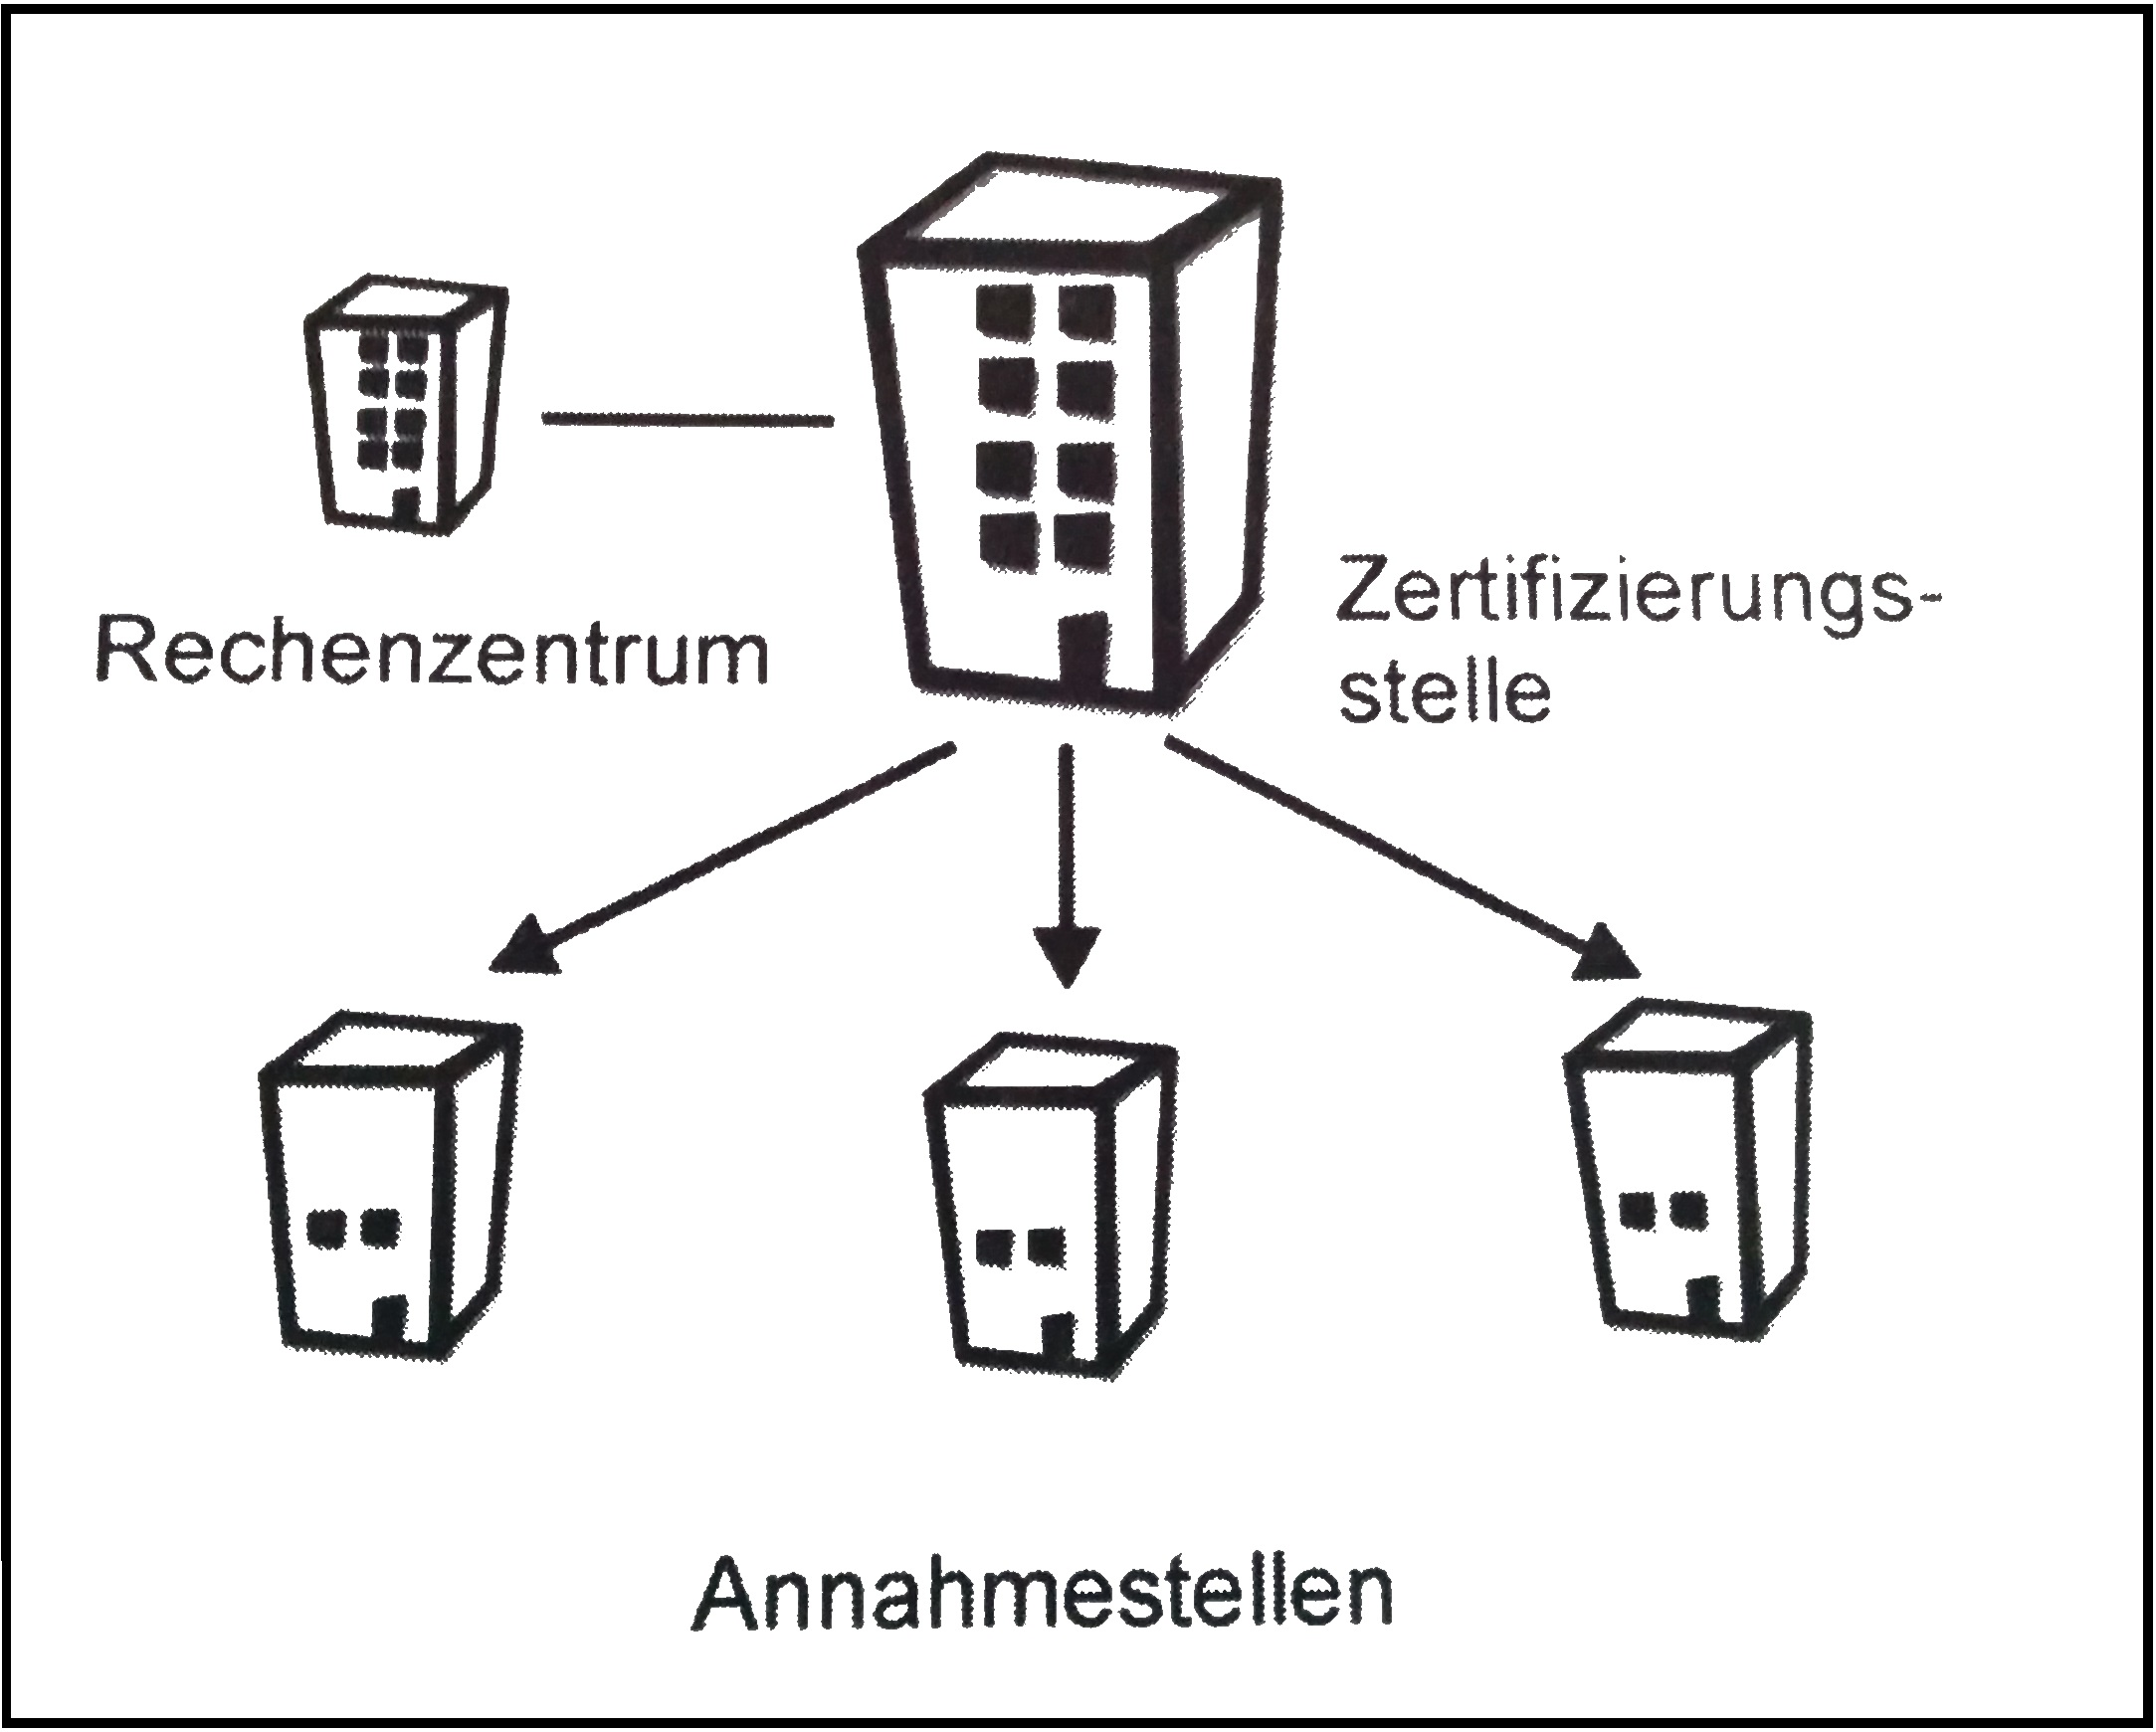
\includegraphics[height=250pt, width=300pt]{trustcenterNeu3.jpg}
    \caption[Schema einer Zertifizierungsstelle]{\small{Schema einer Zertifizierungsstelle \cite{trust1}}}
\end{figure}
\newline
\pagebreak
\textbf{} %Workaround
\newline
Wie auf der Abbildung 1 zu sehen ist, lässt sich die Zertifizierungsstelle in zwei Bereiche einteilen. Auf der einen Seite steht die Annahmestelle, welche die Identifikation der Antragsteller mit Personalausweis und weiteren notariell beglaubigten Dokumenten, z.B. Zulassungen übernehmen. Auf der anderen Seite steht die Zertifizierungsstelle, welche die Erzeugung der Schlüsselpaare und Zertifikate übernimmt. Die Zertifizierungsstelle muss sicherstellen, dass niemand den privaten Schlüssel modifizieren kann. Weiterhin muss der Dienst zur Prüfung der digitalen Signaturen immer verfügbar sein. Abgesehen davon muss sichergestellt werden, dass nur der Antragsteller den privaten Schlüssel erhält. Dies wird meistens mit Chipkarten realisiert. Auf den Chipkarten befindet sich der private Schlüssel und ist vor Auslesung, Manipulation oder Löschung geschützt. Zusätzlich müssen Zertifizierungsstellen noch Dienste, wie die Zulassung von Pseudonyme zur Wahrung des Personlichkeitsrechts des Schlüsselinhabers und ein 24-Stunden-Sperrdienst für Signaturschlüssel anbieten. Des Weiteren muss die Schlüsselaufbewahrung vom Auftraggeber ausdrücklich erklärt werden, ansonsten ist die Speicherung von privaten Schlüsseln in Zertifizierungsstellen nicht erlaubt. Die Pflege des Schlüsselverzeichnis ist von besonderer Bedeutung, da jederzeit die Identifikation von Kommunikationspartnern möglich sein muss. Das Schlüsselverzeichnis muss ständig aktuell und funktionstüchtig sein. Ein weiterer Dienst ist der Zeitstempeldienst. Dieser dient zur genauen Festhaltung, wann ein Dokument erzeugt, verändert oder gelöscht wurde, mittels Zeitangabe der Zertifizierungsstelle im Hashwert für das signierte Dokument. Anwendung findet dieses Verfahren bei der Einhaltung von gesetzlichen Fristen und der Festlegung von Gültigkeitsdauern. \cite{standdeswissens3}\cite{zertstelle1}